%%%%%%%%%%%%%%%%%%%%%
%   AMS packages    %
%%%%%%%%%%%%%%%%%%%%%
\documentclass{amsart}
\usepackage{amsmath}
\usepackage{amsxtra}
\usepackage{amscd}
\usepackage{amsthm}
\usepackage{amsfonts}
\usepackage{amssymb}
\usepackage{eucal}
\usepackage[all]{xy}
\usepackage{graphicx}
\usepackage{comment}
\usepackage{amssymb}
\usepackage{tikz-cd}
\usetikzlibrary{matrix,arrows,decorations.pathmorphing}

\newtheorem{cor}[subsubsection]{Corollary}
\newtheorem{lem}[subsubsection]{Lemma}
\newtheorem{prop}[subsubsection]{Proposition}
\newtheorem{propconstr}{Proposition-Construction}
\newtheorem{ax}{Axiom}
\newtheorem{conj}{Conjecture}
\newtheorem{thm}[subsubsection]{Theorem}
\newtheorem{defn}[subsubsection]{Definition}
\newtheorem{rem}[subsubsection]{Remark}
\newtheorem{eg}[subsubsection]{Example}
\newtheorem{ex}[subsubsection]{Exercise}
\newtheorem{note}[subsubsection]{Notation}
\newtheorem{alg}[subsubsection]{Algorithm}
\newtheorem{fact}[subsubsection]{Fact}

\newcommand\nc{\newcommand}
\nc\on{\operatorname}
\nc\renc{\renewcommand}
\newcommand\ssec{\subsection}
\newcommand\sssec{\subsubsection}
\newcommand\bO{{\mathbf O}}
\newcommand\CC{{\mathcal C}}
\newcommand\BN{{\mathbb N}}
\newcommand\BC{{\mathbb C}}
\newcommand\BF{{\mathbb F}}
\newcommand\BR{{\mathbb R}}
\newcommand\BQ{{\mathbb Q}}
\newcommand\BBZ{{\mathbb Z}}
\newcommand\uR{\underline{R}}
\newcommand\uZ{\underline{\BBZ}}
\newcommand\CF{{\mathcal F}}
\newcommand\uCF{\underline{{\mathcal F}}}
\newcommand\BZ{{\mathbb Z}}
\newcommand\BA{{\mathbb A}}
\newcommand\BP{{\mathbb P}}
\newcommand\fa{{\mathfrak a}}
\newcommand\fp{{\mathfrak p}}
\newcommand\fq{{\mathfrak q}}
\newcommand\fm{{\mathfrak m}}
\newcommand\pt{\mathrm{pt}}
\nc{\bd}{\mathbf{d}}
\nc{\Hom}{\on{Hom}}
\nc{\End}{\on{End}}
\nc{\Spec}{\on{Spec}}
\nc{\Reg}{\on{Reg}}
\nc{\Specm}{\on{Specm}}
\nc\ol{\overline}
\nc\wt{\widetilde}
\nc{\one}{{\mathbf{1}}}
\renc{\mod}{\on{-mod}}
\newcommand{\id}{\mathrm{id}}
\nc{\ul}{\underline}
\nc{\uHom}{\ul\Hom}
\nc{\tHom}{\ul\uHom}
\nc{\wh}{\widehat}
\nc{\Vect}{\on{Vect}}
\nc{\Res}{\on{Res}}
\nc{\Ind}{\on{Ind}}

\newcommand\im{\text{Im}}

\title{Unimodality Ideas}
\author{Aaron Landesman}
\usepackage{amsmath}
\begin{document}

\maketitle
\section{Directions to move}
\begin{enumerate}
	\item Look at generalising $p_i^r$ for general r.
	\item Generalizing to $q$ analog of cyclic group.
	\item Try relating $p_i,q_i.$
	\item Coding which groups $G$ we have $p_i=q_i.$
	\item When are $p_i = q_i.$
	\item Try to compute $q_i.$
	\item Look at simple groups, and maybe solvable groups, try quotienting by normal subgroups?
	\item Are there any ways to combine $G_1,G_2$ where $G_i$ are groups with $p_i = q_i.$
	\item Are there some characterisations of groups with $q_i,p_i.$
	\item How to use sage, what can we do with groups?
	\item Which edge poset definition do we want? Do we include edges containing $y$ or exclude them?
	\item Look at $B_n(q).$ 
	\item Look at generalizing $F_r(B_n)$ to arbitrary posets
	\item Try relating Wilson's Normal Form to our posets?
\end{enumerate}

\section{The Functor of Faces}
\begin{rem}
We assume all posets are ranked posets, and $G$ actions are rank preserving, order preserving actions.
\end{rem}

\begin{defn}
Define the poset category $\mathcal P_r,$ where the objects $P \in \mathcal P_r$ are ranked poset, and the morphisms $Mor(P,Q)$ are rank preserving, order preserving maps, which send all $B_{r+1}$ to other $B_{r+1}$.
\end{defn}

\begin{defn}
Define the {\it Functor of Faces} $\mathcal F:\mathcal P \rightarrow \mathcal P,$ that associates to any poset $P \in \mathcal P$ a poset $\mathcal F(P),$ where the vertices of $\mathcal F(P)$ are pairs $(x,y)\in P \times P,x \lessdot y,$ and the ordering in $\mathcal F(P)$ is given by $(x,y)\leq (a,b)$ if $x \leq a,y\leq b.$ For $f \in Mor(P,Q),$ the corresponding morphism $\mathcal F(f):\mathcal F(P) \rightarrow \mathcal F(Q),$ given by $\mathcal F(f)(x,y) = (f(x),f(y)).$
\end{defn}

\begin{conj}
The Functor of faces $\mathcal F$ is fully faithful.
\end{conj}

\section{Quotient Edges}

This section will build up to the theorem that for a symmetric poset $P,$ with $\mathcal F(P)$ having injective order raising maps for rank $i < \frac{n}{2}$, we will also have $\mathcal F(P/G)$ has injective order raising maps for $i < \frac{n-1}{2}.$ 

\begin{note}
Let $U_i:P_i \rightarrow P_{i+1}$ be the raising operator for the poset $P.$ Then, we obtain an induced map
\begin{align*}
	U_i \otimes U_{i+1}:P_i\otimes P_{i+1} \rightarrow P_{i+1} \otimes P_{i+1},x \otimes y \mapsto U(x) \otimes U(y).
\end{align*}
\end{note}

\begin{note}
We also have the natural inclusions
\begin{align*}
	k_i:\mathcal F(P)_i &\rightarrow P_i \otimes P_{i+1},\\
	x\otimes y &\mapsto x\otimes y\\
	k_i^{G\times G}:\mathcal F(P/G)_i &\rightarrow (P/G)_i \otimes (P/G)_{i+1},\\
	Gx\otimes Gy &\mapsto Gx\otimes Gy,
\end{align*}
where we have $x \lessdot y$ and $Gx \lessdot Gy.$ The maps above are defined on a basis, and are extended by linearity.
\end{note}

\begin{note}
Next, we define the map
\begin{align*}
	j_i:\mathcal (P/G)_i \otimes (P/G)_{i+1} & \rightarrow P_i \otimes P_{i+1},\\
	Gx\otimes Gy &\mapsto \frac{1}{|G|}\sum_{g \in G}^{} gx\otimes \frac{1}{|G|}\sum_{h\in G}^{}hy.
\end{align*}
where $x$ is an arbitrary representative of $Gx$ and $y$ is an arbitrary representative of $Gy$
\end{note}

\begin{lem}
The map $j_i$ is well defined.
\end{lem}
\begin{proof}
It suffices to check that if $x,z$ are two representatives of $Gx,$ then $\sum_{g \in G}^{}gx = \sum_{h \in G}^{}gz.$ This is clear because by definition $Gx = Gz$ means $z = g_1x$ for some $g_1 \in G,$ and so we can reorder the sum.
\end{proof}

\begin{note}
Define the map
\begin{align*}
	p_i: P_i \otimes P_{i+1} &\rightarrow \mathcal (P/G)_i \otimes (P/G)_{i+1},\\
	x\otimes y &\mapsto Gx\otimes Gy.
\end{align*}
\end{note}

\begin{note}
Define the map 
\begin{align*}
	(U_i \otimes U_{i+1})^{G\times G}:P_i\otimes P_{i+1} &\rightarrow P_{i+1} \otimes P_{i+1},\\
	Gx \otimes Gy &\mapsto p_{i+1}\circ(U_i \otimes U_{i+1})\circ j_i(Gx\otimes Gy).
\end{align*}
\end{note}


\begin{note}
We also have the projections inclusions
\begin{align*}
	\pi_i:P_i \otimes P_{i+1} & \rightarrow \mathcal F(P)_{i},\\
	x\otimes y &\mapsto  \begin{cases}
	x\otimes y, &\text{ if }x\lessdot y\\
	0 &\text { otherwise}
\end{cases}\\
	\pi_i^{G\times G}: (P/G)_i \otimes (P/G)_{i+1} &\rightarrow\mathcal F(P/G)_i,\\
	Gx\otimes Gy &\mapsto \begin{cases}
	Gx\otimes Gy, &\text{ if }Gx\lessdot Gy\\
	0 &\text { otherwise}
\end{cases},
\end{align*}
where we have $x \lessdot y$ and $Gx \lessdot Gy.$ The maps above are defined on a basis, and are extended by linearity.
\end{note}

\begin{note}
\label{F_lefchetz}
We denote
\begin{align*}
	\mathcal F(U)_i:\mathcal F(P)_i &\rightarrow \mathcal F(P)_{i+1}\\
	x\otimes y &\mapsto k_i \circ (U \otimes U) \circ \pi_{i+1}(x\otimes y)\\
\mathcal F(U)^{G\times G}_i:\mathcal F(P/G)_i & \rightarrow \mathcal F(P/G)_{i+1}\\
	Gx\otimes Gy &\mapsto k^{G\times G}_i \circ (U \otimes U)^{G\times G} \circ \pi^{G\times G}_{i+1}(Gx\otimes Gy)
\end{align*}
where it is defined above on a basis and we extend to the whole space by linearity.
\end{note}
\begin{rem}
For $i < \frac{n}{2}$ we obtain the following (almost commuting, but $j_{i+1}\circ p_{i+1} \neq \id.$) diagram

\begin{equation}
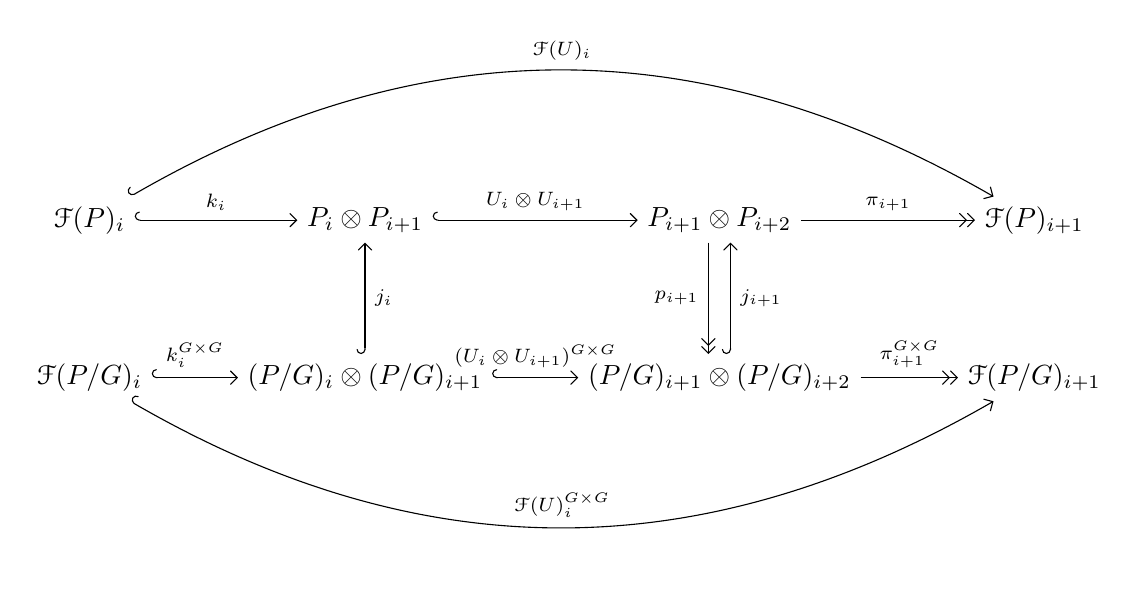
\begin{tikzpicture}[baseline=(current  bounding  box.center)]
\node (a) at (0,0) {$\mathcal F(P)_i$};
\node (b) at (3.5,0) {$P_i \otimes P_{i+1}$};
\node (c) at (8,0) {$P_{i+1} \otimes P_{i+2} $};
\node (d) at (12,0) {$\mathcal F(P)_{i+1}$};
\node (e) at (0,-2) {$\mathcal F(P/G)_i$};
\node (f) at (3.5,-2) {$(P/G)_i \otimes (P/G)_{i+1}$};
\node (g) at (8,-2) {$(P/G)_{i+1} \otimes (P/G)_{i+2} $};
\node (h) at (12,-2) {$\mathcal F(P/G)_{i+1}$};
\path[right hook->,font=\scriptsize,>=angle 90]
([xshift= 4pt]g.north) edge node[right] {$j_{i+1}$} ([xshift= 4pt]c.south)
(a) edge node[above]{$k_i$} (b)
(b) edge node[above]{$U_i\otimes U_{i+1}$} (c)
(e) edge node[above]{$k_i^{G\times G}$}(f)
(f) edge node[above] {$(U_i \otimes U_{i+1})^{G\times G}$} (g)
(f) edge node[right] {$j_{i}$} (b)
(a) edge [bend left] node[above] {$\mathcal F(U)_i$} (d)
(e) edge [bend right] node[above] {$\mathcal F(U)^{G\times G}_i$} (h)
;
\path[->>,font=\scriptsize,>=angle 90]
([xshift= -4pt]c.south) edge node[left] {$p_{i+1}$} ([xshift= -4pt]g.north)
(c) edge node[above] {$\pi_{i+1}$}(d)
(g) edge node[above] {$\pi_{i+1}^{G\times G}$} (h)
;
\end{tikzpicture}
\end{equation}
\end{rem}

\begin{lem}
\label{one_sided_inverse}
The map $p_i$ is a left inverse for $j_i.$ That is, $p_{i}\circ j_{i} = \id.$
\end{lem}
\begin{proof}
For $Gx \otimes Gy \in (P/G)_{i} \otimes (P/G)_{i+1},$ we have
\begin{align*}
	 p_{i}\circ j_{i}(Gx \otimes Gy) &= p_{i}(\frac{1}{|G|}\sum_{g \in G}^{} gx\otimes \frac{1}{|G|}\sum_{h\in G}^{}hy)\\
	 &= \frac{1}{|G|}\sum_{g \in G}^{} Gx\otimes \frac{1}{|G|}\sum_{h\in G}^{}Gy\\
	 &= Gx \otimes Gy
\end{align*}
\end{proof}



\begin{lem}
\label{center_commutes}
 The central square commutes. That is, $j_{i+1} \circ (U_i \otimes U_{i+1})^{G\times G} = (U_i \otimes U_{i+1})\circ j_i.$
\end{lem}
\begin{proof}
By definition, $(U_i \otimes U_{i+1})^{G\times G} = p_{i+1}\circ(U_i \otimes U_{i+1})\circ j_i.$ Therefore, we have $j_{i+1} \circ (U_i \otimes U_{i+1})^{G\times G} = j_{i+1}\circ p_{i+1}\circ(U_i \otimes U_{i+1})\circ j_i.$

So, in order to complete the lemma, it suffices to show that $j_{i+1} \circ p_{i+1}|_{\im((U_i \otimes U_{i+1})\circ j_i)}= \id|_{\im((U_i \otimes U_{i+1})\circ j_i)}.$ Indeed, any element $v \in \im((U_i \otimes U_{i+1})\circ j_i)$ must be of the form 
\begin{align*}
	v=\sum_{x\otimes y}^{}c_{x\otimes y}\left(\frac{1}{|G|}\sum_{g \in G}^{} gx\otimes \frac{1}{|G|}\sum_{h\in G}^{}hy\right).
\end{align*}

In order to show 
\begin{align*}
	j_{i+1} \circ p_{i+1}|_{\im((U_i \otimes U_{i+1})\circ j_i)}= \id|_{\im((U_i \otimes U_{i+1})\circ j_i)},
\end{align*} it suffices to check it on a basis. That is, we only have to show

\begin{align*}
	j_{i+1} \circ p_{i+1}\left(\frac{1}{|G|}\sum_{g \in G}^{} gx\otimes \frac{1}{|G|}\sum_{h\in G}^{}hy\right)= \frac{1}{|G|}\sum_{g \in G}^{} gx\otimes \frac{1}{|G|}\sum_{h\in G}^{}hy,
\end{align*}  or equivalently
\begin{align*}
	j_{i+1} \circ p_{i+1}\left(\sum_{g \in G}^{} gx\otimes \sum_{h\in G}^{}hy\right)= \sum_{g \in G}^{} gx\otimes \sum_{h\in G}^{}hy.
\end{align*}
However,
\begin{align*}
	j_{i+1} \circ p_{i+1}\left(\sum_{g \in G}^{} gx\otimes \sum_{h\in G}^{}hy\right)&= j_{i+1}\left(\sum_{g \in G}^{} Gx\otimes \sum_{h\in G}^{}Gy\right)\\
	&= j_{i+1}\left(|G| \cdot Gx\otimes |G|\cdot Gy\right)\\
	&= \frac{1}{|G|} \sum_{g \in G}^{}|G|gx\otimes \frac{1}{|G|}\sum_{h\in G}^{}|G|hy\\
	&= \sum_{g \in G}^{}gx\otimes\sum_{h\in G}^{}hy
\end{align*}
\end{proof}

\begin{lem}
If $\mathcal F(U)_i$ is injective, then $\ker(\pi_i)|_{\im((U_i \otimes U_{i+1})\circ k_i)}=0.$
\end{lem}
\begin{proof}
Since $\mathcal F(U)_i$ is injective, $\ker \mathcal F(U)_i  = 0.$ Therefore, since $\mathcal F(U)_i = \pi_i \circ (U_i\otimes U_{i+1}) k_i,$ we have $\ker(\pi_i)|_{\im((U_i \otimes U_{i+1})\circ k_i)}=0.$
\end{proof}
THE FOLLOWING PROOF IS WRONG, ITS NOT EXACTLY THE $G$ invariant bases, there are really sums of the G invariant basis. TO FIX THIS, WE REALLY HAVE TO GO UP FIRST, then go right. We can take an averaging when we go up, or we can make an arbitrary choice, it won't matter since $U$ commutes with $G.$ What bothers me is that we only seem to have used that $\mathcal F(U)_i$ is injective, even though it seems that sometimes the quotients aren't injective at the middle.

ALSO, WE MIGHT BE ABLE TO GET PECK POSETS IN GENERAL. I think it has to do with $U_i \otimes U_{i+1}$ being injective from the appropriate levels.

\begin{lem}
\label{no_pi_kernel}
If $\mathcal F(U)_i,$ are injective, then $\ker \pi_{i+1} \cap \im((U\otimes U)\circ j_i\circ k^{G\times G}_i)=0.$
\end{lem}
\begin{proof}
Any element $v \in \im((U\otimes U)\circ j_i\circ k^{G\times G}_i)$ can be written in the form 
\begin{align*}
	v=\sum_{x\otimes y}^{}c_{x\otimes y}\left(\frac{1}{|G|}\sum_{g \in G}^{} gU(x)\otimes \frac{1}{|G|}\sum_{h\in G}^{}hU(y)\right).
\end{align*}

Therefore, if $v \in \ker \pi_{i+1},$ we must have $\pi_{i+1}\left(\frac{1}{|G|}\sum_{g \in G}^{} gU(x)\otimes \frac{1}{|G|}\sum_{h\in G}^{}hU(y)\right) = 0$ for all pairs $(x,y),$ such that $x \in Gx,y \in Gy,$ because distinct orbits are disjoint. BUT WHEN YOU APPLY U THEY ARE NOT DISJOINT! Hence, it suffices to show that we cannot have $\pi_{i+1}\left(\frac{1}{|G|}\sum_{g \in G}^{} gU(x)\otimes \frac{1}{|G|}\sum_{h\in G}^{}hU(y)\right) = 0.$

We know that if $\frac{1}{|G|}\sum_{g \in G}^{} gx\otimes \frac{1}{|G|}\sum_{h\in G}^{}hy \in \im((U\otimes U)\circ j_i\circ k^{G\times G}_i),$ then there must exist some $x \in Gx,y \in Gy$ for which $x \lessdot y.$ However, this implies that $x \otimes y \in Supp\left(\pi_{i+1}\left(\frac{1}{|G|}\sum_{g \in G}^{} gx\otimes \frac{1}{|G|}\sum_{h\in G}^{}hy\right)\right),$ and so in particular $\pi_{i+1}\left(\frac{1}{|G|}\sum_{g \in G}^{} gx\otimes \frac{1}{|G|}\sum_{h\in G}^{}hy\right) \neq 0.$
\end{proof}

\begin{lem}
\label{pi_gg_subset}
We have $\ker \left(\pi^{G\times G}_{i+1}\circ p_{i+1}\right) \cap \im((U\otimes U)\circ j_i\circ k^{G\times G}_i)\subset \ker \pi_{i+1} \cap \im((U\otimes U)\circ j_i\circ k^{G\times G}_i)$
\end{lem}
\begin{proof}
Once, again, starting with an arbitrary $v \in \im((U\otimes U)\circ j_i\circ k^{G\times G}_i),$ we can write
\begin{align*}
	v=\sum_{x\otimes y}^{}c_{x\otimes y}\left(\frac{1}{|G|}\sum_{g \in G}^{} gx\otimes \frac{1}{|G|}\sum_{h\in G}^{}hy\right).
\end{align*}
where $x \lessdot y,$ for all $x \otimes y$ in the support of the above sum. The aim is to show that $v \in \ker \pi \implies v \in \ker (\pi^{G\times G}_i \circ p_i)$ Since distinct $G$ orbits are disjoint, we can assume $v = \frac{1}{|G|}\sum_{g \in G}^{} gx\otimes \frac{1}{|G|}\sum_{h\in G}^{}hy.$ In this case, if $v \in \ker \pi,$ this means $x \not \lessdot y$ for any $x \in Gx,y \in Gy.$ But this means $Gx \not \lessdot Gy,$ and so $v \in \ker (\pi^{G\times G}_i \circ p_i).$ 
\end{proof}

\begin{cor}
\label{no_pi_gg_kernel}
If $\mathcal F(U)_i,$ are injective, then $\ker (\pi^{G\times G}_{i+1}\circ p_{i+1}) \cap \im((U\otimes U)\circ j_i\circ k^{G\times G}_i)=0.$
\end{cor}
\begin{proof}
By ~\ref{pi_gg_subset}, we know $\ker (\pi^{G\times G}_{i+1}\circ p_{i+1}) \cap \im((U\otimes U)\circ j_i\circ k^{G\times G}_i) \subset \ker \pi_{i+1} \cap \im((U\otimes U)\circ j_i\circ k^{G\times G}_i).$ But by ~\ref{no_pi_kernel} we know  $\ker \pi_{i+1} \cap \im((U\otimes U)\circ j_i\circ k^{G\times G}_i)=0.$ Therefore, $\ker (\pi^{G\times G}_{i+1}\circ p_{i+1}) \cap \im((U\otimes U)\circ j_i\circ k^{G\times G}_i)=0.$
\end{proof}

\begin{lem}
\label{injective_chain}
If $\mathcal F(U)_i,U_i,U_{i+1}$ are injective, then so is $\pi^{G\times G}_{i+1}\circ p_{i+1}\circ(U_i\otimes U_{i+1})\circ j_i\circ k^{G\times G}_i.$
\end{lem}
\begin{proof}
Since $U_i,U_{i+1}$ are both injective, $U_i \otimes U_{i+1}$ is as well. It is always the case that $j_i,k^{G\times G}_i$ are injective. Therefore, $(U_i\otimes U_{i+1})\circ j_i\circ k^{G\times G}_i$ is injective. In order to show $\pi^{G\times G}_{i+1}\circ p_{i+1}\circ(U_i\otimes U_{i+1})\circ j_i\circ k^{G\times G}_i$ is injective, it suffices to show that $\ker (\pi^{G\times G}_{i+1}\circ p_{i+1}) \cap \im((U\otimes U)\circ j_i\circ k^{G\times G}_i)=0,$ which is precisely true by ~\ref{no_pi_gg_kernel}
\end{proof}

\begin{lem}
\label{two_equivalent_paths}
We have an equality of linear transformations $\pi^{G\times G}_{i+1}\circ p_{i+1}\circ(U_i\otimes U_{i+1})\circ j_i\circ k^{G\times G}_i = \mathcal F(U)^{G\times G}_i.$
\end{lem}
\begin{proof}
By ~\ref{center_commutes}, we have
\begin{align*}
	\pi^{G\times G}_{i+1}\circ p_{i+1}\circ(U_i\otimes U_{i+1})\circ j_i\circ k^{G\times G}_i = \pi^{G\times G}_{i+1}\circ p_{i+1}\circ j_{i+1}\circ(U_i\otimes U_{i+1})^{G\times G}\circ k^{G\times G}_i.
\end{align*}

Then, by ~\ref{one_sided_inverse}, we obtain
\begin{align*}
	\pi^{G\times G}_{i+1}\circ p_{i+1}\circ j_{i+1}\circ(U_i\otimes U_{i+1})^{G\times G}\circ k^{G\times G}_i &= \pi^{G\times G}_{i+1}\circ(U_i\otimes U_{i+1})^{G\times G}\circ k^{G\times G}_i\\
	&= \mathcal F(U)^{G\times G}_i
\end{align*}
Therefore,
\begin{align*}
	\pi^{G\times G}_{i+1}\circ p_{i+1}\circ(U_i\otimes U_{i+1})\circ j_i\circ k^{G\times G}_i = \mathcal F(U)^{G\times G}_i.
\end{align*}
\end{proof}

\begin{thm}
\label{injectivity_thm}
If $\mathcal F(U)_i,U_i,U_{i+1}$ are injective, then $\mathcal F(U)^{G\times G}_i$ is injective.
\end{thm}
\begin{proof}
By ~\ref{injective_chain}, we know $\pi^{G\times G}_{i+1}\circ p_{i+1}\circ(U_i\otimes U_{i+1})\circ j_i\circ k^{G\times G}_i$ is injective. But by ~\ref{two_equivalent_paths}, $\pi^{G\times G}_{i+1}\circ p_{i+1}\circ(U_i\otimes U_{i+1})\circ j_i\circ k^{G\times G}_i = \mathcal F(U)_i.$ Therefore, $\mathcal F(U)_i$ is injective.
\end{proof}

\section{The object $\mathcal F(B_n).$}

\begin{note}
For this section, we will use $L = \mathcal F(U)^{n-2i-1},$ where $\mathcal F(U)^{n-2i-1}:\mathcal F(B_n)_i \rightarrow \mathcal F(B_n)_{n-i-1}$ is the lefchetz map, as defined in ~\ref{F_lefchetz}.
\end{note}
\begin{note}
For the remainder of this section, we shall take $|a| = n-i-1,|b|= n-i,|x| = i,|y| = i+1.$ Additionally, whenever we write an expression of the form $x \otimes y$ or $a \otimes b,$ it is assumed that $x \lessdot y,a \lessdot b.$
\end{note}


\begin{thm}
The map $L$ satisfies 
\begin{align*}
	L(x\otimes y) =(2^k - 1)(k-1)! \sum_{y \not \subset a,x\subset a,y \subset b}^{}a \otimes b + k!\sum_{|b| = n-i,|a| = n-i-1,a \lessdot b,y \subset a}^{}a \otimes b
\end{align*}
\end{thm}
\begin{proof}
COME BACK TO THIS THEOREM (MAYBE SOMEONE ELSE CAN WRITE IT UP.)
\end{proof}

\begin{thm}
The poset $P_n$ whose vertices are pairs $x\otimes y,x \lessdot y,$ and whose relations are $x\otimes y < a\otimes b$ if $y\setminus x = b\setminus a,$ defines a poset which is isomorphic to a disjoint union of $n$ copies of $B_{n-1}.$ Therefore it is unitary peck. Furthermore, composing its lefchetz map $n-2i-1$ times yields $M:(P_n)_i \rightarrow (P_n)_{n-i-1},$ such that $M(x\otimes y)	 = k!\sum_{|b| = n-i,|a| = n-i-1,a \lessdot b,y \subset a}^{}a \otimes b$
\end{thm}
\begin{proof}

COME BACK TO THIS THEOREM (MAYBE SOMEONE ELSE CAN WRITE IT UP.)
\end{proof}


\ssec{Proof that $B_n$ is peck}

The aim of this proof will be to show that the matrix produced above is invertible.

\section{The proof from the row point of view}

In this section, we will show the rows of $L$ form a basis by showing we can make a change of basis to a map which is a Lefchetz map on a disjoint union of $n$ copies of $B_{n-1}.$ Since $B_{n-1}$ is unitary peck, it will follow that $L$ is an isomorphism.

\begin{note}

Let $\beta = \frac{2^k-1}{k}.$ Denote 
\begin{align*}
	v_{a \otimes b} =\beta \sum_{y \subset a}^{}x \otimes y + \sum_{y\subset b,x \subset a,y\not\subset a}^{}x\otimes y.
\end{align*}
Note that $v_{a \otimes b}$ are simply the rows of $L,$ each divided by the constant $k!.$
\end{note}

\begin{note}
For any set $s$ of size at least $n-i,$
\begin{align*}
	z_s = \frac{1}{\beta\binom {|s|-i-1}{n-2i-2}(|s|-n+i+1)+\binom{|s|-i-1}{n-2i-1}} \sum_{b\subset s,a \subset b}^{}v_{a\otimes b}
\end{align*}
\end{note}



\begin{lem}
\label{z_equivalence}
For any set $s$ of size at least $n-i,$ we have $z_s = \sum_{y \subset s}^{}x\otimes y.$ In particular, $\sum_{y \subset s}^{}x\otimes y$ lies in the span of $v_{a\otimes b}$
\end{lem}
\begin{proof}
We have 
\begin{align*}
	&\left(\beta\binom {|s|-i-1}{n-2i-2}(|s|-n+i+1)+\binom{|s|-i-1}{n-2i-1}\right) z_s \\
	&= \sum_{b\subset s,a \subset b}^{}v_{a\otimes b}\\
	&=\sum_{b\subset s,a \subset b}^{} \left(\beta \sum_{y \subset a}^{}x \otimes y + \sum_{y\subset b,x \subset a,y\not\subset a}^{}x\otimes y.\right)\\
	&= \sum_{b\subset s,a \subset b}^{} \beta \sum_{y \subset a}^{}x \otimes y + \sum_{b\subset s,a \subset b}^{} \sum_{y\subset b,x \subset a,y\not\subset a}^{}x\otimes y.\\
	&= \beta\binom {|s|-i-1}{n-2i-2}(|s|-n+i+1) \sum_{y \subset s}^{}x \otimes y+ \sum_{b\subset s,a \subset b}^{} \sum_{y\subset b,x \subset a,y\not\subset a}^{}x\otimes y.\\
	&= \beta\binom {|s|-i-1}{n-2i-2}(|s|-n+i+1) \sum_{y \subset s}^{}x \otimes y + \binom{|s|-i-1}{n-2i-1}\sum_{y\subset s}^{}x\otimes y\\
	& =\left(\frac{1}{\beta\binom {|s|-i-1}{n-2i-2}(|s|-n+i+1)+\binom{|s|-i-1}{n-2i-1}}\right) \sum_{y \subset s}^{}x\otimes y.
\end{align*}
In going between the fourth line and the fifth line, I counted the number of $y$ satisfying $y \subset a \subset b\subset s.$ If we fix $s,a$ there are $(|s|-n+i+1)$ choices for the element $b,$ since it can add any element in $s$ but not in $a.$ Then, we need to count the number of $a$ with $y \subset a \subset s.$ This is exactly $\binom {|s|-i-1}{n-2i-2}(|s|-n+i+1).$

In going from the fifth line to the sixth line, for $y,s$ fixed, we count the number of $b$ with $y \subset b \subset s.$ This is exactly $\binom{|s|-i-1}{n-2i-1}$.
\end{proof}

\begin{note}
For any set $s$ of size at least $n-i,$ let $w_s = \sum_{a \subset s,t\notin s}^{}v_{a \otimes a \cup \{t\}}.$
\end{note}

\begin{lem}
\label{w_equivalence}
We have 
\begin{align*}
	w_s = \sum_{t\notin s}^{} \left(\beta \binom {|s|-i-1}{n-2i-2}	\sum_{y \subset s}^{}x\otimes x \cup \{t\}  + \binom {|s|-i}{n-2i-1} \sum_{x \subset s}^{}x \otimes x \cup \{t\} \right).
\end{align*}
\end{lem}

\begin{proof}
\begin{align*}
	w_s &= \sum_{a \subset s,t\notin s}^{}v_{a \otimes a \cup \{t\}}\\
	&= \sum_{a \subset s,t\notin s}^{}\left(\beta \sum_{y \subset a}^{}x \otimes y + \sum_{y\subset b,x \subset a,y\not\subset a \cup \{t\}}^{}x\otimes y \right)\\
	&= \sum_{t\notin s}^{}\left(\sum_{a \subset s}^{}\beta \sum_{y \subset a}^{}x \otimes y + \sum_{a \subset s}^{}\sum_{y\subset b,x \subset a,y\not\subset a \cup \{t\}}^{}x\otimes y \right)\\
	&=\sum_{t\notin s}^{}\left(\beta \binom {|s|-i-1}{n-2i-2}\sum_{y \subset s}^{}x\otimes y + \sum_{a \subset s}^{}\sum_{y\subset b,x \subset a,y\not\subset a \cup \{t\}}^{}x\otimes y \right)\\
	&=\sum_{t\notin s}^{} \left(\beta \binom {|s|-i-1}{n-2i-2}\sum_{y \subset s}^{}x\otimes y + \binom {|s|-i}{n-2i-1}\sum_{x \subset s}^{}x \otimes x \cup \{t\} \right)
\end{align*}
The equalities between lines three and four, and four and five hold for similar reasons as the equalities between lines four and five, and five and six in ~\ref{z_equivalence}
\end{proof}

\begin{note}
Let $u_s = \frac{w_s - (n - |s|)\beta \binom {|s|-i-1}{n-2i-2} z_s}{\binom {|s|-i}{n-2i-1}} + z_s.$
\end{note}

\begin{lem}
\label{u_equivalence}
We have $u_s = \sum_{x\subset s,y\supset x}^{}x\otimes y.$ In particular, $\sum_{x\subset s,y\supset x}^{}x\otimes y$ lies in the span of $v_{a\otimes b}.$
\end{lem}
\begin{proof}
By ~\ref{w_equivalence} and ~\ref{z_equivalence} we have
\begin{align*}
	u_s &= \frac{w_s - (n - |s|)\beta \binom {|s|-i-1}{n-2i-2} z_s}{\binom {|s|-i}{n-2i-1}} + z_s\\
	&= \frac{\sum_{t\notin s}^{} \left(\beta \binom {|s|-i-1}{n-2i-2}\sum_{y \subset s}^{}x\otimes y + \binom {|s|-i}{n-2i-1}\sum_{x \subset s}^{}x \otimes x \cup \{t\} \right) - (n - |s|)\beta \binom {|s|-i-1}{n-2i-2} \sum_{y \subset s}^{}x\otimes y}{\binom {|s|-i}{n-2i-1}} + \sum_{y \subset s}^{}x\otimes y \\
	&=  \frac{\sum_{t\notin s}^{} \left(\sum_{x \subset s}^{}x \otimes x \cup \{t\} \right)}{\binom {|s|-i}{n-2i-1}} + \sum_{y \subset s}^{}x\otimes y \\
	&= \sum_{t\notin s}^{} \left(\binom {|s|-i}{n-2i-1}\sum_{x \subset s}^{}x \otimes x \cup \{t\} \right) + \sum_{y \subset s}^{}x\otimes y \\
	&=  \sum_{x\subset s,y\supset x}^{}x\otimes y
\end{align*}
The penultimate line is equal to the ultimate line because any element $x\otimes y$ with $x \subset s$ must either have $y \subset s$ or else $y \subset s \cup \{t\}$ for $t \notin s.$ The two terms on the penultimate line cover precisely these two cases.
\end{proof}

\begin{note}
For any $s \subset [n],$ with $|s| \leq n-i,$ define $h_s = z_{[n]} - u_s.$
\end{note}

\begin{lem}
\label{h_equivalence}
With $h_s$ as defined above $h_s = \sum_{x\not\subset s}^{}x\otimes y$
\end{lem}
\begin{proof}
Using ~\ref{z_equivalence} and ~\ref{u_equivalence}
\begin{align*}
	h_s &= z_{[n]} - u_s \\
	&= \sum_{x\subset y}^{}x\otimes y-\sum_{x\subset s,x\subset y}^{}x\otimes y\\
	&= \sum_{x\not\subset s}^{}x\otimes y
\end{align*}
\end{proof}
\begin{note}
For $I \subset[n],$ let $I^c = [n]\setminus I,$ the complement of $I$ in $[n].$
\end{note}


\begin{note}
For $I,J$ with $I\subset J \subset [n],$ and $I \neq \emptyset.$ such that $|J| \leq i,$ define $l_{J,I}= \sum_{x \supset J, J \cap x = I}^{}x\otimes y.$
\end{note}

\begin{lem}
\label{l_base_case}
Assuming $i \neq 0,$ for $|s| = n-1,$ it follows that $h_s = l_{s^c,s^c}.$
\end{lem}
\begin{proof}
By ~\ref{h_equivalence},
\begin{align*}
	h_s &=\sum_{x\not\subset s}^{}x\otimes y\\
  	&=\sum_{s^c \subset x}^{} x\otimes y\\
  	&=l_{s^c,s^c}
\end{align*}
In equating the first line with the second line, we are crucially using that $|s^c| = 1,$ because then $x \not \subset s \Leftrightarrow s^c \subset x.$ 
\end{proof}

\begin{lem}
\label{l_induction_step}
$l_{s^c,s^c} = h_s - \sum_{I \subset s^c, I \neq s^c,I \neq\emptyset}^{}l_{s^c,I}.$
\end{lem}
\begin{proof}
We have
\begin{align*}
	h_s & = \sum_{x\not\subset s}^{}x\otimes y\\
	&= \sum_{x\cap s^c \neq \emptyset}^{}x\otimes y\\
	&= \sum_{I \subset s^c,I \neq \emptyset,x\cap s^c = I}^{}x\otimes y\\
	&= \sum_{x\cap s^c = s^c}^{}x\otimes y+\sum_{I \subset s^c,I \neq s^c,I \neq \emptyset,x\cap s^c = I}^{}x\otimes y\\
	&= l_{s^c,s^c} + \sum_{I \subset s^c, I \neq s^c,I \neq \emptyset}^{}l_{s^c,I}
\end{align*}
\end{proof}

\begin{lem}
For all $J \subset [n],$ with $|J| \leq i,$ we have $l_{J,J}$ lies in the span of $v_{a \otimes b}.$ 
\end{lem}
\begin{proof}
By ~\ref{l_base_case} we have that for any $s,|s| = n-1,$ we have $l_{s^c,s^c}$ lies in the span of $v_{a\otimes b}.$ Inductively assume that we have shown $l_{s^c,s^c}$ lies in the span of $v_{a\otimes b}$ for $|s| > j.$ Then, for $|s| = j$ we can use ~\ref{l_induction_step} to write $l_{s^c,s^c}$ in terms of $h_s$ and $l_{r^c,r^c}$ where $|r|>j.$ Since we know both  $h_s$ and $l_{r^c,r^c}$ lie in the span of $v_{a\otimes b},$ so does $l_{s^c,s^c}$ for all $s,|s| > n-i.$
\end{proof}

\begin{lem}
\label{l_diag_equivalence}
For $|x| = i,$ we have $l_{x,x} = \sum_{y \supset x}^{}y\otimes x.$
\end{lem}
\begin{proof}
By definition, $l_{\bar x,\bar x} = \sum_{\bar x\subset x,\bar x \cap x = \bar x,x\subset y}^{}x\otimes y = \sum_{\bar x\subset y}^{}\bar x\otimes y.$ Replacing $\bar x$ by $x$ gives the result.
\end{proof}

\begin{note}
Define $m_a = \sum_{x \subset a}^{}l_{x,x}.$
\end{note}

\begin{lem}
With $m_a$ as defined above, we have $m_a = \sum_{x\subset a}^{}x\otimes y.$
\end{lem}
\begin{proof}
By ~\ref{l_diag_equivalence}, we obtain
$$m_a = \sum_{x \subset a}^{}l_{x,x} = \sum_{x \subset a}^{}\sum_{y \supset x}^{}y\otimes x= \sum_{x\subset a}^{}x\otimes y$$
\end{proof}

\begin{note}
Denote $r_a = \sum_{b,b\subset a}^{} a \otimes b.$
\end{note}

\begin{lem}
With $r_a$ as defined above, we have $r_a = C_1\sum_{y\subset a}^{}x\otimes y + C_2 \sum_{x\subset a}^{}x\otimes y.$
\end{lem}
\begin{proof}

\end{proof}
\begin{note}

Define $t_a = \frac{r_a - C_2 m_a}{C_1} = \sum_{y\subset a}^{}x\otimes y $
\end{note}

\begin{note}
Let $q_{a,b} = v_{a\otimes b} - t_a.$
\end{note}

\begin{lem}
We have $q_{a,b} = \sum_{y\subset b,x \subset a,y\not\subset a}^{}x\otimes y.$
\end{lem}
\begin{proof}

\end{proof}

\begin{thm}
The matrix $L$ is invertible.
\end{thm}
\begin{proof}
We saw that $q_{a,b} = \sum_{y\subset b,x \subset a,y\not\subset a}^{}x\otimes y$ lie in the span of $v_{a\otimes b}.$ However, $q_{a,b}$ are exactly the rows of a lefchetz map on a disjoint union of $n$ copies of $B_{n-1}.$ Since the lefchetz map on $B_{n-1}$ is invertible, this means the $q_{a,b}$ form a basis for $\mathcal F(B_n)_{i}$ and therefore the $v_{a\otimes b}$ do as well. Therefore, $L$ is invertible. 
\end{proof}



\begin{lem}
With $t_a$ as defined above, $t_a = \frac{r_a - C_1 m_a}{C_2}.$
\end{lem}
\begin{proof}

\end{proof}



\end{document}